%<dscrpt>Fichier de déclarations Latex à inclure au début d'un élément de cours.</dscrpt>

\documentclass[a4paper]{article}
\usepackage[hmargin={1.8cm,1.8cm},vmargin={2.4cm,2.4cm},headheight=13.1pt]{geometry}

%includeheadfoot,scale=1.1,centering,hoffset=-0.5cm,
\usepackage[pdftex]{graphicx,color}
\usepackage[french]{babel}
%\selectlanguage{french}
\addto\captionsfrench{
  \def\contentsname{Plan}
}
\usepackage{fancyhdr}
\usepackage{floatflt}
\usepackage{amsmath}
\usepackage{amssymb}
\usepackage{amsthm}
\usepackage{stmaryrd}
%\usepackage{ucs}
\usepackage[utf8]{inputenc}
%\usepackage[latin1]{inputenc}
\usepackage[T1]{fontenc}


\usepackage{titletoc}
%\contentsmargin{2.55em}
\dottedcontents{section}[2.5em]{}{1.8em}{1pc}
\dottedcontents{subsection}[3.5em]{}{1.2em}{1pc}
\dottedcontents{subsubsection}[5em]{}{1em}{1pc}

\usepackage[pdftex,colorlinks={true},urlcolor={blue},pdfauthor={remy Nicolai},bookmarks={true}]{hyperref}
\usepackage{makeidx}

\usepackage{multicol}
\usepackage{multirow}
\usepackage{wrapfig}
\usepackage{array}
\usepackage{subfig}


%\usepackage{tikz}
%\usetikzlibrary{calc, shapes, backgrounds}
%pour la présentation du pseudo-code
% !!!!!!!!!!!!!!      le package n'est pas présent sur le serveur sous fedora 16 !!!!!!!!!!!!!!!!!!!!!!!!
%\usepackage[french,ruled,vlined]{algorithm2e}

%pr{\'e}sentation du compteur de niveau 2 dans les listes
\makeatletter
\renewcommand{\labelenumii}{\theenumii.}
\renewcommand{\thesection}{\Roman{section}.}
\renewcommand{\thesubsection}{\arabic{subsection}.}
\renewcommand{\thesubsubsection}{\arabic{subsubsection}.}
\makeatother


%dimension des pages, en-t{\^e}te et bas de page
%\pdfpagewidth=20cm
%\pdfpageheight=14cm
%   \setlength{\oddsidemargin}{-2cm}
%   \setlength{\voffset}{-1.5cm}
%   \setlength{\textheight}{12cm}
%   \setlength{\textwidth}{25.2cm}
   \columnsep=1cm
   \columnseprule=0.5pt

%En tete et pied de page
\pagestyle{fancy}
\lhead{MPSI-\'Eléments de cours}
\rhead{\today}
%\rhead{25/11/05}
\lfoot{\tiny{Cette création est mise à disposition selon le Contrat\\ Paternité-Pas d'utilisations commerciale-Partage des Conditions Initiales à l'Identique 2.0 France\\ disponible en ligne http://creativecommons.org/licenses/by-nc-sa/2.0/fr/
} }
\rfoot{\tiny{Rémy Nicolai \jobname}}


\newcommand{\baseurl}{http://back.maquisdoc.net/data/cours\_nicolair/}
\newcommand{\urlexo}{http://back.maquisdoc.net/data/exos_nicolair/}
\newcommand{\urlcours}{https://maquisdoc-math.fra1.digitaloceanspaces.com/}

\newcommand{\N}{\mathbb{N}}
\newcommand{\Z}{\mathbb{Z}}
\newcommand{\C}{\mathbb{C}}
\newcommand{\R}{\mathbb{R}}
\newcommand{\D}{\mathbb{D}}
\newcommand{\K}{\mathbf{K}}
\newcommand{\Q}{\mathbb{Q}}
\newcommand{\F}{\mathbf{F}}
\newcommand{\U}{\mathbb{U}}
\newcommand{\p}{\mathbb{P}}


\newcommand{\card}{\mathop{\mathrm{Card}}}
\newcommand{\Id}{\mathop{\mathrm{Id}}}
\newcommand{\Ker}{\mathop{\mathrm{Ker}}}
\newcommand{\Vect}{\mathop{\mathrm{Vect}}}
\newcommand{\cotg}{\mathop{\mathrm{cotan}}}
\newcommand{\sh}{\mathop{\mathrm{sh}}}
\newcommand{\ch}{\mathop{\mathrm{ch}}}
\newcommand{\argsh}{\mathop{\mathrm{argsh}}}
\newcommand{\argch}{\mathop{\mathrm{argch}}}
\newcommand{\tr}{\mathop{\mathrm{tr}}}
\newcommand{\rg}{\mathop{\mathrm{rg}}}
\newcommand{\rang}{\mathop{\mathrm{rg}}}
\newcommand{\Mat}{\mathop{\mathrm{Mat}}}
\newcommand{\MatB}[2]{\mathop{\mathrm{Mat}}_{\mathcal{#1}}\left( #2\right) }
\newcommand{\MatBB}[3]{\mathop{\mathrm{Mat}}_{\mathcal{#1} \mathcal{#2}}\left( #3\right) }
\renewcommand{\Re}{\mathop{\mathrm{Re}}}
\renewcommand{\Im}{\mathop{\mathrm{Im}}}
\renewcommand{\th}{\mathop{\mathrm{th}}}
\newcommand{\repere}{$(O,\overrightarrow{i},\overrightarrow{j},\overrightarrow{k})$}
\newcommand{\cov}{\mathop{\mathrm{Cov}}}

\newcommand{\absolue}[1]{\left| #1 \right|}
\newcommand{\fonc}[5]{#1 : \begin{cases}#2 \rightarrow #3 \\ #4 \mapsto #5 \end{cases}}
\newcommand{\depar}[2]{\dfrac{\partial #1}{\partial #2}}
\newcommand{\norme}[1]{\left\| #1 \right\|}
\newcommand{\se}{\geq}
\newcommand{\ie}{\leq}
\newcommand{\trans}{\mathstrut^t\!}
\newcommand{\val}{\mathop{\mathrm{val}}}
\newcommand{\grad}{\mathop{\overrightarrow{\mathrm{grad}}}}

\newtheorem*{thm}{Théorème}
\newtheorem{thmn}{Théorème}
\newtheorem*{prop}{Proposition}
\newtheorem{propn}{Proposition}
\newtheorem*{pa}{Présentation axiomatique}
\newtheorem*{propdef}{Proposition - Définition}
\newtheorem*{lem}{Lemme}
\newtheorem{lemn}{Lemme}

\theoremstyle{definition}
\newtheorem*{defi}{Définition}
\newtheorem*{nota}{Notation}
\newtheorem*{exple}{Exemple}
\newtheorem*{exples}{Exemples}


\newenvironment{demo}{\renewcommand{\proofname}{Preuve}\begin{proof}}{\end{proof}}
%\renewcommand{\proofname}{Preuve} doit etre après le begin{document} pour fonctionner

\theoremstyle{remark}
\newtheorem*{rem}{Remarque}
\newtheorem*{rems}{Remarques}

\renewcommand{\indexspace}{}
\renewenvironment{theindex}
  {\section*{Index} %\addcontentsline{toc}{section}{\protect\numberline{0.}{Index}}
   \begin{multicols}{2}
    \begin{itemize}}
  {\end{itemize} \end{multicols}}


%pour annuler les commandes beamer
\renewenvironment{frame}{}{}
\newcommand{\frametitle}[1]{}
\newcommand{\framesubtitle}[1]{}

\newcommand{\debutcours}[2]{
  \chead{#1}
  \begin{center}
     \begin{huge}\textbf{#1}\end{huge}
     \begin{Large}\begin{center}Rédaction incomplète. Version #2\end{center}\end{Large}
  \end{center}
  %\section*{Plan et Index}
  %\begin{frame}  commande beamer
  \tableofcontents
  %\end{frame}   commande beamer
  \printindex
}


\makeindex
\begin{document}
\noindent

\debutcours{Probabilités sur un univers fini}{0.2}

\section{Expérience aléatoire et univers probabilisé}
\subsection{Expérience aléatoire.}
Une expérience aléatoire n'est pas un objet mathématique mais une situation réelle qui conduit à plusieurs issues possibles. Elle est décrite en langage usuel et cette description peut souvent s'interpréter de diverses manières. On choisit de modéliser ces issues par un ensemble mathématique appelé \emph{univers}. \newline
Souvent la description de l'expérience n'est pas assez précise pour assurer l'unicité d'un univers pertinent. Le traitement mathématique ne s'occupe pas de ce problème et commence \emph{après} que le modèle soit choisi. On se limite ici aux expériences aléatoires modélisées par des univers \emph{finis}.\newline
Une fois l'univers choisi, il est \emph{probabilisé} c'est à dire muni d'une certaine fonction de probabilté souvent notée $\p$ défini dans un certain ensemble de parties et à valeur dans $[0,1]$. Il peut être intéressant de considérer plusieurs modèles différents pour la même expérience aléatoire et de comparer les résultats obtenus; on trouvera souvent les mêmes.\newline
Certains concepts attachés aux expériences aléatoires correspondent à des objets mathématiques de la théorie des ensembles. On propose un dictionnaire.
\subsection{Dictionnaire.}
\begin{center}
\begin{tabular}{ll}
Univers (fini) &  Ensemble (fini) \\
\'Evénement & Partie   \\
\'Evénement élémentaire (issue) & Singleton \\ 
\'Evénement contraire & Complémentaire \\
\'Evénement \og $A$ et $B$\fg & $A\cap B$ (intersection) \\
\'Evénement \og $A$ ou $B$\fg & $A\cup B$ (union) \\
\'Evénement imposssible & partie vide $\emptyset$ \\
\'Evénements incompatibles & Parties disjointes \\
Système complet d'événements & Partition
\end{tabular} 
\end{center}

\subsection{Espace probabilisé fini.}
\begin{defi}
 Une probabilité sur un univers fini $\Omega$ est une fonction $\p$ définie sur $\mathcal{P}(\Omega)$ et à valeurs dans $[0,1]$ telle que:
\begin{displaymath}
 \p(\Omega) = 1, \hspace{1cm} \forall (A,B)\in \mathcal{P}(\Omega)^2, \hspace{0.5cm} A\cap B = \emptyset \Rightarrow \p(A\cup B) = \p(A) + \p(B)
\end{displaymath}
\end{defi}
Dans un univers fini, on peut définir une fonction probabilité par les images des singletons. Comme toutes les parties sont finies et que les singletons sont deux à deux disjoints:
\begin{displaymath}
\forall A\in \mathcal{P}(\Omega), \; \p(A) = \sum_{a\in A} \p(\left\lbrace a \right\rbrace )
\end{displaymath}

\begin{prop}Probabilité de l'union.
 \begin{displaymath}
\forall (A,B) \in \mathcal{P}(E)^2, \; \p(A\cup B) = \p(A) + \p(B) - \p(A\cap B)  
 \end{displaymath}
\end{prop}
\begin{demo}
 On écrit les unions disjointes
\begin{multline*}
\left. 
\begin{aligned}
 A =& (A\cap \overline{B}) \cup (A\cap B) \\ B =& (B\cap \overline{A}) \cup (A\cap B)\\ A \cup B =& (A\cap \overline{B}) \cup (B\cap \overline{A}) \cup (A\cap B) 
\end{aligned}
\right\rbrace \Rightarrow
\left. 
\begin{aligned}
 \p(A) =& \p(A\cap \overline{B}) + \p(A\cap B) \\ \p(B) =& \p(B\cap \overline{A}) + \p(A\cap B)\\ 
 \p(A \cup B) =& \p(A\cap \overline{B}) + \p(B\cap \overline{A}) + \p(A\cap B)
\end{aligned}
\right\rbrace \\
\Rightarrow \p(A \cup B) = \p(A) + \p(B) - \p(A\cap B)
\end{multline*}
\end{demo}

Probabilité de l'événement contraire.
\begin{displaymath}
 \p(A) + \p(\overline{A}) = 1
\end{displaymath}

Croissance.
\begin{displaymath}
\forall (A,B)\in \mathcal{P}(\Omega)^2, \hspace{0.5cm} A\subset B \Rightarrow \p(A) \leq \p(B) 
\end{displaymath}

Exercice.(\href{\urlexo _fex_pb.pdf}{pb05 feuille Probabilités sur un espace fini}) Formule du crible à partir de la formule pour la fonction caractéristique de l'union de $p$ parties.
Soit $(A_1, \cdots, A_n)$ une famille d'évènements:
\[
 \p(\bigcup_{i \in \llbracket 1, n \rrbracket}) =
 \sum_{k=1}^{n}\left( (-1)^{k+1}\sum_{I \in \mathcal{P}_k(\llbracket 1, n \rrbracket)}\p(A_I)\right) 
 \hspace{1cm} \text{ avec } 
 A_I = \bigcap_{k \in I} A_k .
\]


\section{Espaces probabilisés usuels.}
En général, dans les exercices, l'univers probabilisé modélisant l'expérience aléatoire n'est pas donné. On propose ici quelques espaces probalisés usuels qui peuvent servir à modéliser les expériences aléatoires rencontrées assez souvent.

Pour une fonction probabilisé uniforme, l'univers est en général formé à partir d'un ensemble usuel du dénombrement. Les fonctions probabilités non uniformes apparaissent dans des expériences aléatoires complexes; c'est à dire composées de plusieurs sous-expériences plus simples. Il est commode alors d'utiliser comme univers un ensemble de chemins dans un arbre.

\subsection{Probabilité uniforme}
\begin{defi}
 Une probabilité est dite uniforme lorsque tous les événements élémentaires sont équiprobables. La probabilité d'un événement élementaire est alors $\frac{1}{n}$ où $n$ est le cardinal de l'univers.
\end{defi}
\begin{prop}
  Si $p$ est une probabilité uniforme sur un univers fini $\Omega$, pour tout événement $A$:
\begin{displaymath}
  \p(A) = \frac{\sharp A}{\sharp \Omega}
\end{displaymath}
\end{prop}
Dans un espace probabilisé uniforme, ce qui est important c'est que l'ensemble mathématique décrive bien les issues de l'expérience. Les calculs de probabilités se ramènent à des dénombrements. On utilise souvent les ensembles suivants
\begin{itemize}
 \item Ensembles de parties.
\begin{itemize}
  \item parties à $p$ éléments dans un ensemble à $32$ éléments pour modéliser les \og mains\fg~ de $p$ cartes tirées d'un jeu de 32.
  \item parties à moins de 2 éléments dans un ensemble de 6 éléments pour modéliser des dominos.
  \item tirage simultané d'objets.
\end{itemize}
 
 \item Ensembles de fonctions.
 \begin{itemize}
   \item fonctions de $\llbracket 1,n\rrbracket$ dans $\llbracket 1,p\rrbracket$  pour modéliser les distributions  de $n$ objets à $p$ personnes ou des tirages avec remise de $n$ objets dans un ensemble de $p$.
   \item ensemble de fonctions injectives pour une succession de tirages sans remise.
   \item ensemble de fonctions pour une succession de tirages avec remise.
 \end{itemize}
 \item Ensembles de solutions d'équations du type $x_1+\cdots+x_p=n$ avec des contraintes sur les inconnues $x_i$.
\end{itemize}

Que faire avec des expériences dont les issues ne sont pas équiprobables?
\begin{itemize}
  \item Si les issues sont des nombres, on peut chercher parmi des \og modèles numériques usuels\fg~ un modèle satisfaisant. Cela revient en fait à la considération de \emph{lois usuelles} de variables aléatoires.
  \item Si l'expérience est trop complexe pour correspondre à des espaces probabilisés usuels, il faut chercher à la décomposer en expériences plus simples jusqu'à arriver à des expériences élémentaires pour lesquelles l'équiprobabilité est vérifiée. On obtient alors un modèle qui se décrit avec des graphes orientés. Cela revient à modéliser des \emph{probabilités conditionnelles}.
\end{itemize}

\subsection{Composition d'expériences aléatoires. Graphes orientés}
On considère des expériences aléatoires qui sont composées de plusieurs expériences aléatoires qui se suivent et qui peuvent dépendre des précédentes. Les expériences aléatoires les plus élémentaires sont probabilisées de manière uniforme. Le processus de l'expérience se modélise à l'aide d'un graphe \emph{orienté} connexe.\newline
On peut caractériser ce graphe par les propriétés suivantes:
\begin{itemize}
  \item L'ensemble des sommets est fini (donc l'ensemble des arêtes aussi).
  \item Il existe une unique sommet (\emph{l'origine}) qui n'est l'arrivée d'aucune arête (valence entrante nulle) et qui est le départ d'au moins deux arêtes (valence sortante $\geq2$).
  \item Il existe des sommets particuliers (les feuilles ou les sorties) qui ne sont le départ d'aucune arête (valence sortante nulle).
  \item Le graphe ne contient aucun circuit c'est à dire un chemin partant d'un sommet et y retournant.
\end{itemize}

Les sommets (sauf l'origine) représentent un état du système, les arêtes sortantes pointent vers les nouveaux états qui sont les issues d'une expérience aléatoire élémentaire.  Les ensembles de feuilles ou les ensembles de chemins vers les feuilles de certains graphes orientés et pondérés permettent de bien décrire certaines expériences aléatoires qui \emph{se décomposent} en expériences élémentaires.
Quels graphes ? Quelle pondération ?
\begin{defi}
  L'ensemble des chemins de la racine aux feuilles d'un tel graphe est probabilisé par une pondération des arêtes. Cette pondération doit vérifier les propriétés suivantes.
\begin{itemize}
  \item Tous les poids sont positifs ou nuls.
  \item La somme des poids des arêtes issues d'un même noeud est égale à 1.
  \item La probabilité d'un chemin est le produit des poids des arêtes qui le constituent.
\end{itemize}
 L'ensemble des feuilles est alors aussi probabilisé. La probabilité élémentaire d'une feuille est la somme des probabilités des chemins qui y mènent.
\end{defi}

On considère par exemple le tirage sans remise de deux boules dans une urne qui contient deux boules noires et deux boules blanches. Trois issues sont possibles mais comme elles ne sont pas équiprobables, le modèle le plus commode pour cette expérience est l'ensemble des chemins de la figure suivante
\begin{figure}[h!]
 \centering
 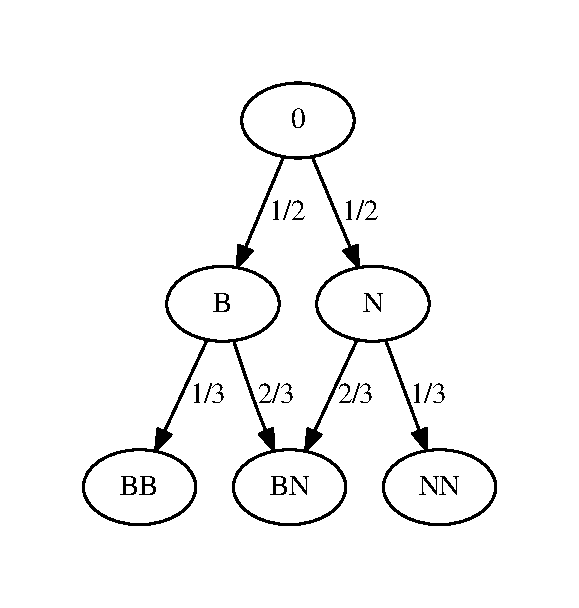
\includegraphics{./C9646_1.pdf}
 % C9646_1.pdf: 0x0 pixel, 0dpi, 0.00x0.00 cm, bb=
\end{figure}

Un exemple d'expérience aléatoire mal définie : deux personnes entrent dans un parc dans lequel se trouvent  3 bancs à 2 places. Quelle est la probabilité qu'ils s'assoient sur le même banc? On trouve $\frac{1}{5}$ ou $\frac{1}{3}$ selon que l'on envisage les places ou les bancs.


\subsection{Espaces probabilisés numériques.}
On considère des expériences aléatoires dont les issues sont des \emph{nombres} (en général des nombres naturels). L'univers probabilisé est alors une partie finie de $\N$ munie d'une probabilité qui n'est pas uniforme. On propose quelques modèles usuels d'espaces probabilisés de ce type. Attention seuls les modèles de Bernoulli et binomial sont au programme de MPSI. 
\subsubsection{Modèle de Bernoulli.}
\begin{defi}
  Soit $p\in [0,1]$. Le modèle de Bernoulli de paramètre $p$ est l'ensemble $\{0,1\}$ probabilisé par :
  \begin{displaymath}
    \text{la probabilité de } \{0\} = 1-p,\hspace{1cm} \text{la probabilité de } \{1\} = p
  \end{displaymath}
\end{defi}
\begin{rems}
\begin{itemize}
  \item Toute expérience aléatoire qui n'a que deux issues est bien décrite par un modèle de Bernoulli. On peut convenir d'appeler  \og de Bernoulli\fg~ une telle expérience.
  \item Attention à ne pas confondre le $p$ du paramètre avec le nom de la fonction probabilité.
\end{itemize}
\end{rems}

\subsubsection{Modèle binomial.}
\begin{defi}
  Soit $p\in [0,1]$ et $n\in \N^*$. Le modèle binomial de paramètres $n$, $p$ est l'ensemble $\llbracket 0 , n \rrbracket$ probabilisé par :
  \begin{displaymath}
    \forall k \in \llbracket 0 , n \rrbracket, \; \text{la probabilité de } \{k\} = \binom{k}{n}p^k(1-p)^{n-k}
  \end{displaymath}
\end{defi}
Si on répète $n$ fois une expérience de Bernoulli de paramètre $p$, on obtient une expérience complexe que l'on peut décrire à l'aide d'un graphe. Il s'agit en fait d'un arbre \emph{binaire} de longueur $n$. Chaque arête correspond à l'issue $0$ (pondérée par $1-p$) ou $1$ (pondérée par $p$) d'une expérience de Bernoulli, Dans ce cas, il s'agit bien d'un vrai arbre avec un seul chemin pour aller vers une feuille donnée.\newline
La probabilité d'un chemin particulier est $p^k(1-p)^{n-p}$ où $k$ est le nombre fois où l'expérience élémentaire a donné $1$. Si on s'intéresse seulement au nombre de fois où le $1$ a été obtenu, l'ensemble des issues est $\llbracket 0, n \rrbracket$ et la probabilité du singleton $\{k\}$ est le nombre de chemins multiplié par la probabilité d'un chemin convenable soit $\binom{k}{n}p^k(1-p)^{n-k}$.



\section{Probabilités conditionnelles}
\index{probabilité conditionnelle}
Soit $p$ une probabilité et $B$ un événement possible $\p(B)>0$. La fonction
\begin{displaymath}
 \left\lbrace 
\begin{aligned}
 \mathcal{P}(\Omega) &\rightarrow [0,1] \\
 A &\mapsto \frac{\p(A\cap B)}{\p(B)}
\end{aligned}
\right. 
\end{displaymath}
est une probabilité notée $P_B$. On note aussi $\p(A|B)$ et on parle de \emph{probabilité conditionnelle} de $A$ sachant $B$.

\index{formule des probabilités composées}
\begin{prop}[Formule des probabilités composées]
 Soit $(A_1,\cdots,A_n)$ des événements tels que $\p(A_1\cap \cdots \cap A_n)>0$ alors
\begin{displaymath}
 \p(A_1\cap \cdots \cap A_n) = \p(A_1)p_{A_1}(A_2)p_{A_1\cap A_2}(A_3) \cdots p_{A_1\cap \cdots A_{n-1}}(A_n)
\end{displaymath}
\end{prop}
\begin{demo}
  Le produit se simplifie en dominos multiplicatifs.
\end{demo}


\index{formule des probabilités totales}
\begin{prop}[Formule des probabilités totales]
Soit $(A_1,\cdots,A_n)$ un système complets d'événements de probabilités non nulles, alors: 
\begin{displaymath}
\forall B\in \mathcal{P}(\Omega),\hspace{0.5cm} \p(B) = \sum_{i=1}^{n}\p(B\cap A_i) = \sum_{i=1}^{n}p_{A_i}(B)\p(A_i)
\end{displaymath}
\end{prop}
\begin{demo}
  La formule traduit la décomposition de $B$ en une réunion disjointe $B = \cup_{i=1}^{n}(B\cap A_i)$.
\end{demo}

\index{formules de Bayes}
\begin{prop}[Formules de Bayes]
 Soient $A$ et $B$ deux événements tels que $\p(A)>0$ et $\p(B)>0$,
\begin{displaymath}
 \p(A|B) = \frac{\p(B|A)\p(A)}{\p(B)}
\end{displaymath}
Si $(A_1,\cdots,A_n)$ est un système complets d'événements de probabilités non nulles et si $B$ est un événement de probabilité non nulle, alors
\begin{displaymath}
 \p(A_j|B) = \frac{\p(B|A_j) \p(A_j)}{\sum_{i=1}^n\p(B|A_i)\p(A_i)}
\end{displaymath}
\end{prop}
\begin{demo}
  La formule de Bayes est une conséquence directe de la définition d'une probabilité conditionnelle.
\begin{displaymath}
  \p(A|B) = \frac{\p(A\cap B)}{\p(B)} = \frac{\p(B|A)\, \p(A)}{\p(B)}
\end{displaymath}
Pour la deuxième formule, on utilise la formule des probabilités totales:
\begin{displaymath}
\left. 
\begin{aligned}
\p(A_j \cap B) &= \p(B| A_j)\p(_j) \\
\p(B) &= \sum_{i=1}^{n}\p(B\cap A_i)
\end{aligned}
\right\rbrace \Rightarrow
\p(A_j|B) = \frac{\p(A_j \cap B)}{\p(B)} = \frac{\p(B| A_j)\p(_j)}{\sum_{i=1}^{n}\p(B\cap A_i)}
\end{displaymath}
\end{demo}


\section{\'Evénements indépendants}
\begin{defi}
Dans un espace probabilisé par $p$, deux événements $A$ et $B$ sont dits indépendants si et seulement si 
\begin{displaymath}
  \p(A\cap B) = \p(A)\p(B)
\end{displaymath}  
\end{defi}
\begin{rem}
 La justification du terme \og indépendant\fg vient de ce que deux évènements $A$ et $B$ sont indépendants si et seulement si la probabilité de $A$sachant $B$ est égale à la probabilité de $A$ : $\p_B(A) = \p(A)$.
\end{rem}

\begin{prop}
  $A$ et $B$ indépendants entraîne $(A,\overline{B})$, $(\overline{A},B)$, $(\overline{A},\overline{B})$ indépendants.
\end{prop}
\begin{demo}
Soit $A$ et $B$ deux événements indépendants. D'après la formule donnant la probabilité de l'événement contraire:
\begin{displaymath}
  \p(A)\p(\overline{B})=\p(A)(1-\p(B)) = \p(A) - \p(A)\p(B) = \p(A) - \p(A\cap B) = \p(A \cap (\overline{A\cap B}) = \p(A \cap \overline{B})
\end{displaymath}
On obtient l'autre formule en intervertissant les rôles de $A$ et $B$ puis en remplaçant $B$ et $\overline{B}$ puisque $A$ et $\overline{B}$ sont aussi indépendants.
\end{demo}
\begin{defi}
Dans un espace probabilisé par $p$, les événements d'une famille $A_1,\cdots,A_n$ sont dits \emph{deux à deux indépendants} si et seulement si p 
\begin{displaymath}
  \forall (i,j)\in \llbracket 1,n \rrbracket^2,\; i\neq j \Rightarrow \p(A_i \cap a_j) = \p(A_i)\p(A_j)
\end{displaymath}  
\end{defi}

\begin{defi}
Dans un espace probabilisé par $\p$, les événements d'une famille $A_1,\cdots,A_n$ sont dits \emph{mutuellement indépendants} si et seulement si pour toute partie $I$ de $\llbracket 1,n \rrbracket$, 
\begin{displaymath}
  p\left( \bigcap_{i\in I}A_i\right)  = \prod_{i\in I}\p(A_i)
\end{displaymath}  
\end{defi}
\begin{exple}
  Une famille d'événements deux à deux indépendants mais non mutuellement indépendants.\newline
On lance deux fois une pièce et on considère les trois événements:
\begin{itemize}
  \item $A$: pile au premier lancer.
  \item $B$: face au deuxième lancer.
  \item $C$: le même résultat aux deux lancers.
\end{itemize}
On trouve 
\begin{displaymath}
  \p(A)= \p(B) = \p(C) = \frac{1}{2},\hspace{0.5cm} \p(A\cap B)= \p(B \cap C) = \p(A \cap C) = \frac{1}{4},\hspace{0.5cm} \p(A \cap B \cap C) = 0
\end{displaymath}
\end{exple}

\end{document}

